\documentclass[11pt,a4paper]{article}

\usepackage[T1]{fontenc}
\usepackage[utf8]{inputenc}
\usepackage[english]{babel}
\usepackage{lmodern}
%\usepackage{circuitikz}
\usepackage{color}
\usepackage{wrapfig}
\usepackage{placeins}
\usepackage{subfigure}
\usepackage{tabu}
\usepackage{fullpage}
\usepackage[squaren]{SIunits}
\usepackage{graphicx}
%\usepackage[pdftex]{graphicx}
\usepackage{epstopdf}
\usepackage{epsfig}
\usepackage{hyperref}
\usepackage{tikz}
\usepackage{tikz-qtree}
\usepackage{eurosym}
%\usepackage{chemist}
\usepackage{amsmath}
\usepackage{amssymb}
\usepackage{mathrsfs}
\usepackage{dsfont}% use $\mathds{1}$
\newcommand{\C}{\mathbb{C}}
\newcommand{\N}{\mathbb{N}}
\newcommand{\Z}{\mathbb{Z}}
\newcommand{\R}{\mathbb{R}}
\newcommand{\red}{\textcolor{red}}
\newcommand{\dis}{\displaystyle}
\newcommand{\dr}{\partial}
\newcommand{\txt}{\text}
\newcommand{\td}{\todo[inline]}
\newcommand{\ttt}{\texttt}
\newcommand{\itt}{\textit}

\usepackage{algorithm}
\usepackage{todonotes}
\usepackage[noend]{algpseudocode}

%\newtheorem{theoreme}			     {Théorème}	[chapter]
%\newtheorem{proposition}[theoreme]	 {Proposition}	
%\newtheorem{corollaire}	  [theoreme]	 {Corollaire}	
%\newtheorem{lemme}	      [theoreme]  {Lemme}		
%\newtheorem{definition}	         {Définition}[chapter]
%\theoremstyle{definition}
%\newtheorem{exemple}			     {Exemple}	[chapter]
%\newtheorem{contreexemple}[exemple]{Contre-exemple}
%\newtheorem{probleme}	             {Probl\`eme}[chapter]

\usepackage{listings}
\usepackage{textcomp}
\definecolor{listinggray}{gray}{0.9}
\definecolor{lbcolor}{rgb}{0.9,0.9,0.9}
\lstset{
	backgroundcolor=\color{lbcolor},
	tabsize=4,
	rulecolor=,
	language=matlab,
        basicstyle=\scriptsize,
        upquote=true,
        aboveskip={1.5\baselineskip},
        columns=fixed,
        showstringspaces=false,
        extendedchars=true,
        breaklines=true,
        prebreak = \raisebox{0ex}[0ex][0ex]{\ensuremath{\hookleftarrow}},
        frame=single,
        showtabs=false,
        showspaces=false,
        showstringspaces=false,
        identifierstyle=\ttfamily,
        keywordstyle=\color[rgb]{0,0,1},
        commentstyle=\color[rgb]{0.133,0.545,0.133},
        stringstyle=\color[rgb]{0.627,0.126,0.941},
}

\DeclareMathOperator{\e}{e}

\title{Titre}
\author{David Weicker}
\date{\today}

\begin{document}
\tabulinesep=1.2mm
\begin{center}
\hrule
\begin{tabular}{c}
\\[0.005cm]
\Large{Insert Title Here}\\[0.3cm] %THIS IS THE TITLE
\textsc{NAME1} name1  \& \textsc{NAME2} name2\\[0.2cm]
$\text{6}^{\text{th}}$ November 2015\\[0.2cm] %THIS IS THE DATE
\end{tabular}
\hrule
\end{center}

\section{Model 1}
The telecommunication company Nett provides capacity between cites in Europe. The cities are Stockholm, Berlin, London, Warsaw, Paris, Madrid and Rome. Some of the cities are connected in which traffic can be sent in both directions. The connections and the maximum traffic which can be sent between the cites respectively can be seen in Figure 1.

Nett wishes to provide 50 Gbit/s between Stockholm and Rome at the same time they provide 40 Gbit/s between London and Warsaw. They need help in routing the traffic because of the capacity limitations. Also, they would like to investigate if there is any slack in the network, potential to adding another traffic route and how to handle fluctuations in capacity.

\begin{center}
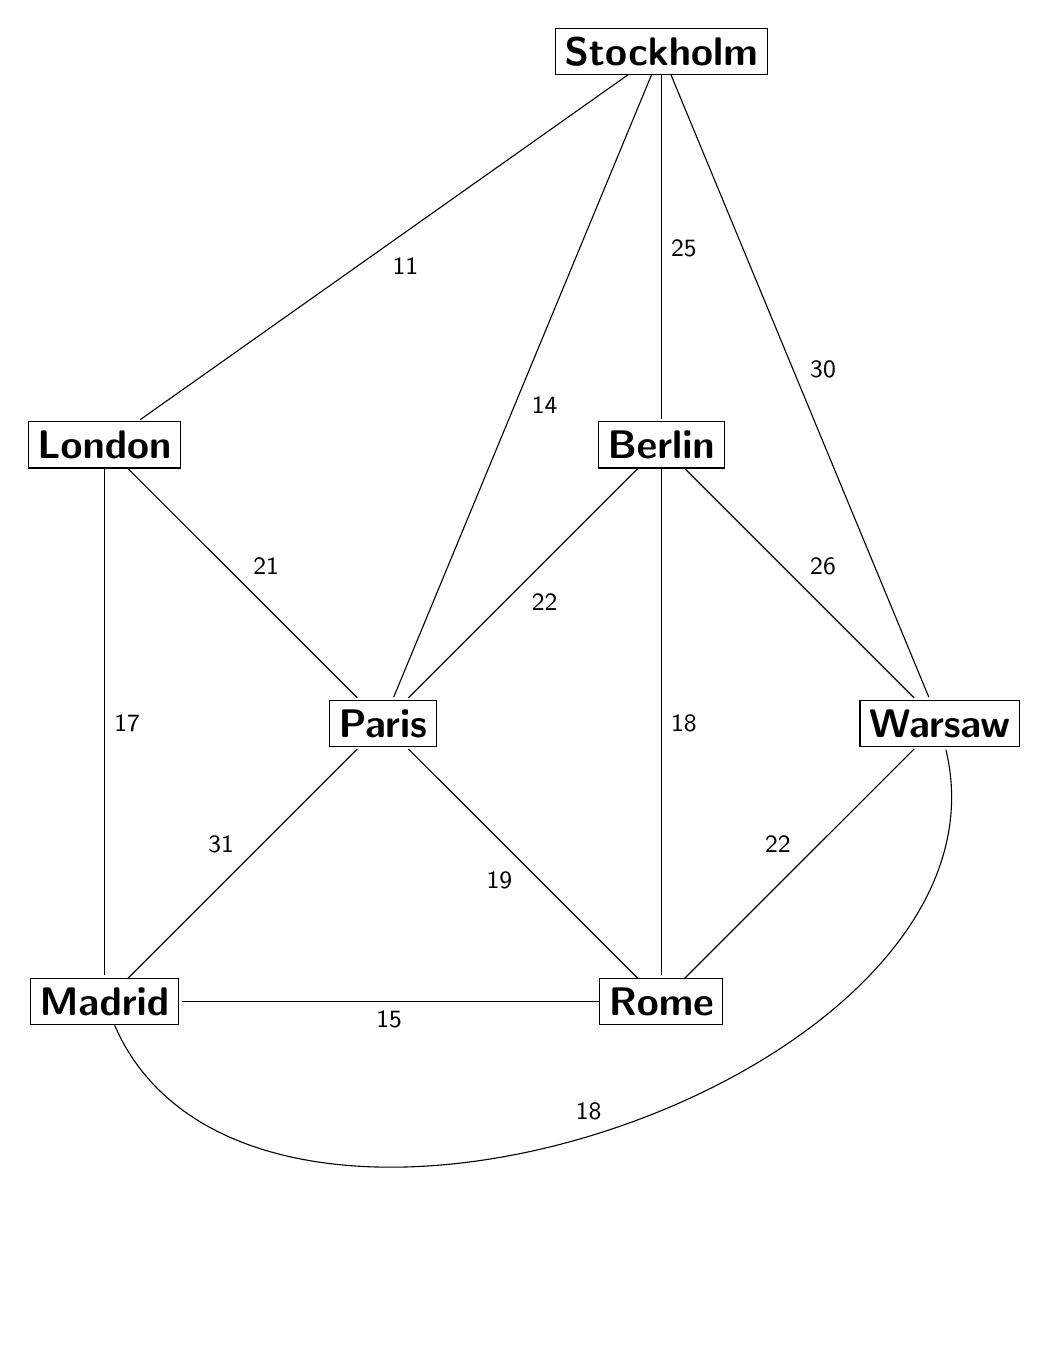
\begin{tikzpicture}[shorten >=1pt,auto,node distance=5cm,
                    main node/.style={rectangle,draw,font=\sffamily\Large\bfseries}]
  \node[main node] (1) {Stockholm};
  \node[main node] (2) [below of=1] {Berlin};
  \node[main node] (3) [below right of=2] {Warsaw};
  \node[main node] (4) [below left of=2] {Paris};
  \node[main node] (5) [above left of=4] {London};
  \node[main node] (6) [below right of=4] {Rome};
  \node[main node] (7) [below left of=4] {Madrid};

  \path[every node/.style={font=\sffamily\small}]
    (1) edge node {25} (2)
     	edge node {30} (3)
    	edge node {14} (4)
    	edge node {11} (5)
    (2) edge node {26} (3)
    	edge node {22} (4)
        edge node {18} (6)
    (5) edge node {17} (7)
        edge node {21} (4)
    (6) edge node {19} (4)
        edge node {15} (7)
        edge node {22} (3)
    (7) edge [bend right=85] node {18} (3)
    	edge node {31} (4);
  
\end{tikzpicture}
\end{center}
Figure 1. System modelled as a network where maximum capacity is marked out on the arcs.

\newpage

\section*{Routing the traffic}

\begin{center}
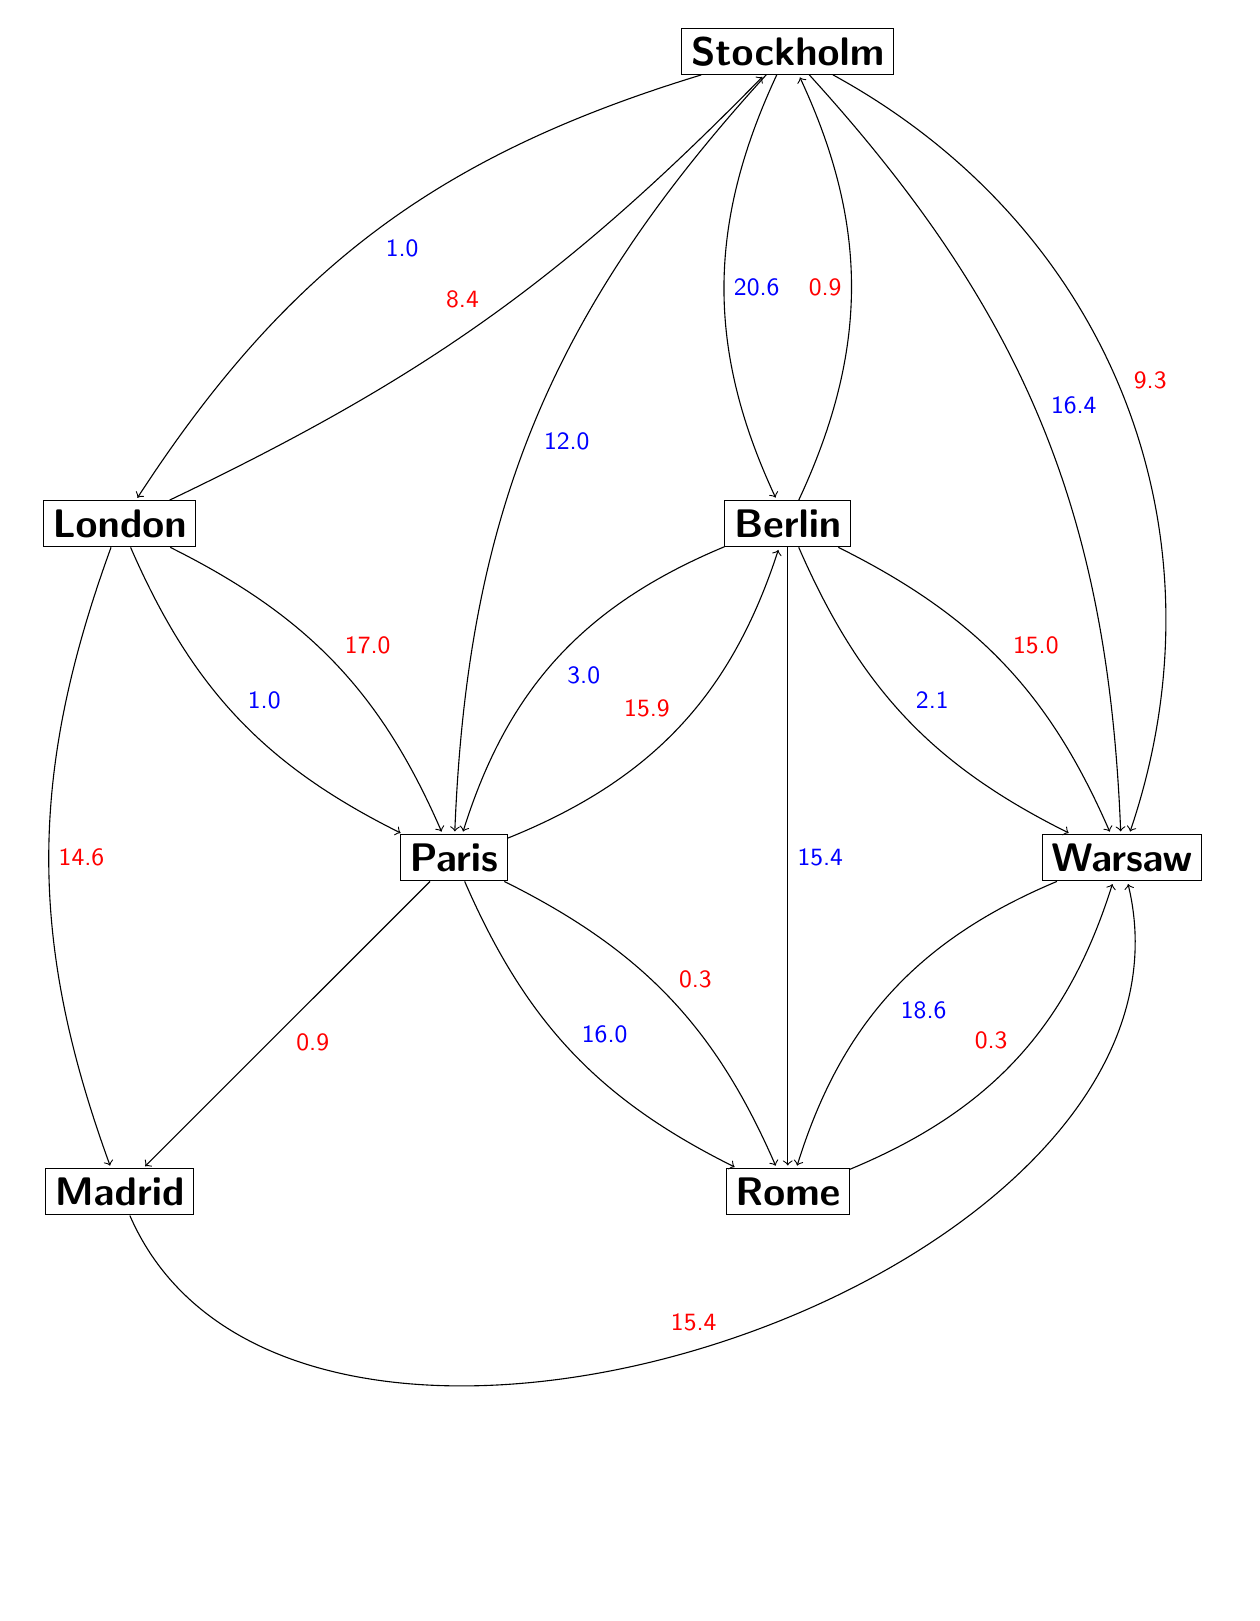
\begin{tikzpicture}[->,shorten >=1pt,auto,node distance=6cm,
                    main node/.style={rectangle,draw,font=\sffamily\Large\bfseries}]
  \node[main node] (1) {Stockholm};
  \node[main node] (2) [below of=1] {Berlin};
  \node[main node] (3) [below right of=2] {Warsaw};
  \node[main node] (4) [below left of=2] {Paris};
  \node[main node] (5) [above left of=4] {London};
  \node[main node] (6) [below right of=4] {Rome};
  \node[main node] (7) [below left of=4] {Madrid};

  \path[every node/.style={font=\sffamily\small}]
    (1) edge [bend right=20] node[blue] {1.0} (5)
    	edge [bend right=20] node[blue] {12.0} (4)
     	edge [bend right=25] node[blue] {20.6} (2)
    	edge [bend left=20] node[blue] {16.4} (3)
    	edge [bend left=40] node[red] {9.3} (3)
    (2) edge [bend right=25] node[red] {0.9} (1)
    	edge [bend right=25] node[blue] {3.0} (4)
        edge [bend right=20] node[blue] {2.1} (3)
    	edge [bend left=20] node[red] {15.0} (3)
    	edge node[blue] {15.4} (6)
    (3) edge [bend right=25] node[blue] {18.6} (6)
    (4) edge [bend right=25] node[red] {15.9} (2)
    	edge [bend right=20] node[blue] {16.0} (6)
    	edge [bend left=20] node[red] {0.3} (6)
    	edge node[red] {0.9} (7)
    (5) edge [bend right=10] node[red] {8.4} (1)
    	edge [bend left=20] node[red] {17.0} (4)
    	edge [bend right=20] node[blue] {1.0} (4)
		edge [bend right=20] node[red] {14.6} (7)
	(6) edge [bend right=25] node[red] {0.3} (3)
    (7) edge [bend right=85] node[red] {15.4} (3);
  
\end{tikzpicture}
\end{center}

\section{Model 2}
blibli

\section{Model 3}
\subsection{Presentation of the problem}
In this section, we are going to generalize the model a little bit. Up to this point, we have considered that each link has a known capacity and that this quantity is exact. This is, however, not true in general. We can expect the actual capacities to be close to the numbers given but we should take into account that they can fluctuate around those values. Our new model will thus have to deal with this uncertainty. Because the value of the capacities can be considered as an unknown parameter, we will use stochastic programming.

We also know that the 50 Gbit/s-demand can be rerouted after the actual values are known but the 40 Gbit/s-demand must be determined on beforehand (and thus not cannot be rerouted after knowing the actual capacities).

\subsection{Mathematical model}
Just as in the previous models, we introduce the set $I$ :
$$I = \{ Sto,Lon,Ber,War,Par,Rom,Mad\}$$


 



\end{document}